\part{ R3BRoot User Guide }
\chapter{Parameters }
\label{chap:intro}
\minitoc

\section{ Introduction}
%-----------------------

\subsection{ ROOT and VMC  }

Here i write about general blabla framework

\begin{figure}[!htbp]
  \begin{center}
    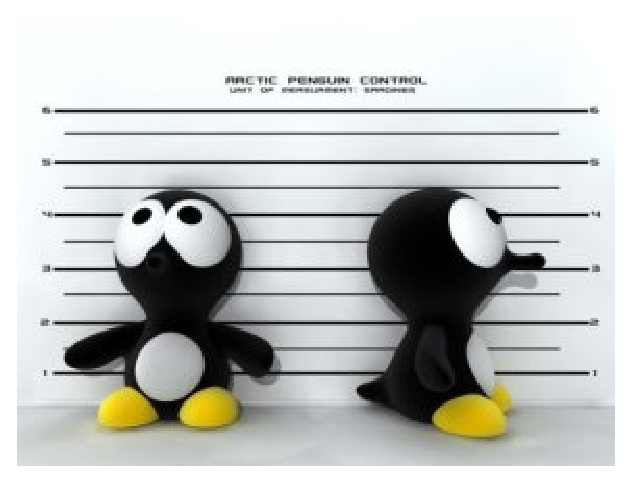
\includegraphics[width=0.9\textwidth]{Chapitre1/arctic_control}
  \end{center}
  \caption{A nice image...}
  \label{fig:jolieImage}
\end{figure}

\subsection{ The FairRoot framework }

Here is some general ideas about FairRoot, etc ... 


\section{Getting started}
%------------------------

\subsection{ Installation }

Here is more about installing things in GSI 
or external. \\
Running some basics example macros. \\  
Inspecting the results. \\

%\begin{equation}
%  T = \argmin_T E(T,R,F)
%\end{equation}


\subsection{ Running a Simulation example}
%-------------------------------------

Here more about example macros etc... \\

Showing a great bullet list environment:

\subsection{Accessing results}

Here more about Root Trees , Stack simple analysis macros \\
Also Event Diplay stuff ... briefly ...

%\begin{bulletList}
% \item First point
% \item Second point
% \item Here is an abbreviation reference \nomenclature{DTI}{Diffusion Tensor Imaging} DTI
%\end{bulletList}

\chapter{geometry}
\chapter{transport model}

